\documentclass[a4paper,11pt,pdf]{pacmanreport}

%%=== Aditional packages
\usepackage{amsmath}
\usepackage{amsfonts}

% The following is used to make packages hyperref and cite work together
\makeatletter
\let\NAT@parse\undefined
\makeatother
\usepackage[bookmarks=true,hyperfootnotes=true,colorlinks=true,linkcolor=blue,anchorcolor=blue,citecolor=blue,urlcolor=blue,filecolor=blue]{hyperref}

%%=== Local definitions
\graphicspath{{images/}{../shared_images/}}

%% ================================
%% PROJECT INFO

\project{}
\projectid{FP7-IST-60918}
\projectstart{1 March 2013}
\duration{36}

%% ================================
%% DELIVERABLE INFO

\title{Methodologies for incipient grasp evaluation}
\deliverableid{DR 4.2}
\author{H. Marino, M. Bonilla, C. Rosales, M. Kopicki, C. Zito, J.L.~Wyatt, M. Gabiccini}
\address{Universit\`{a} di Pisa, Pisa Italy}
\email{m.gabiccini@ing.unipi.it}
\headertitle{Incipient grasp}
\headerauthor{H. Marino, M. Bonilla, C. Rosales, M. Kopicki, C. Zito, J. Wyatt, M. Gabiccini}

\duedate{2015-02-28}
\submissiondate{2015-02-28}
\leadpartner{Universit\`{a} di Pisa}
\revision{draft}
\disseminationlevel{PU}


%% UNCOMMENT: to get the logo; if you've copied this file to a directory yearX/wpY/ then this should work
\reportlogo{pacmanlogo.png}


\begin{document}

\maketitle

\begin{abstract}
\noindent This report describes the activities related to the control of grasping actions given the detection of an object. It includes work on: modelling underactuated and adaptive robotic hands, acquiring target grasps learned from data gathered either from humans or simulations, synthesising grasps for novel objects using either heuristic or statistical machine learning approaches, planning complex grasping and manipulation tasks either using discrete search methods or via direct trajectory optimization methods for systems with unspecified contact sequences.
\end{abstract}


\vspace{.2em}
\hrule

\footnotesize

\tableofcontents

\normalsize

\newpage

\section*{Executive Summary}

This report describes the activities --- most of which already performed, while some others scheduled for finalization in the weeks that precede the PaCMan review meeting in May 2015 --- within the PaCMan consortium to define methodologies for \emph{incipient grasping evaluation}. The material included in this report describes the results that fall under Task 4.2 (M 7-18), and the progress of Task 4.3 (M 7-30) at M 24.

\section*{Role of incipient grasps evaluation in PaCMan}

This deliverable documents the effort of the consortium in devising new strategies to define \emph{practical} approaches to tackle the problem of \emph{grasping under uncertainty}, either caused by clutter, visual occlusions, and new object shapes. To this sake, the ability to evaluate \emph{incipient grasps} in terms of their expected quality, robustness, and probability of success, is of paramount importance.

\section*{Contribution to the PaCMan scenario}

To our eyes, grasp methodologies that try to cope with pose uncertainty, object shape estimation inaccuracies, clutter and partial occlusions, either (i) by accomodating grasp unmodelled dynamics by exploiting prior knowledge about the adaptivity and the compliance of the Pisa/IIT SoftHand (as mainly proposed by the UNIPI Team), or (ii) by inferring grasps for novel objects from as little as one training example (of a chosen grasp type) that are shown to be generalizable within and \emph{across} object categories, even with partial shape information, (as mainly proposed by The UoB Team), represent central contributions in the scenario depicted in the PaCMan project.


\newpage

\section{Tasks, objectives, results}

\subsection{Planned work}

Humans have no troubles in selecting the correct grasp strategies even if the object to be grasped is unknown or partially visible. On the contrary, though robotics has made significant progress in the field of autonomous grasping, the problem of grasping novel objects in cluttered scenarios has not been completely solved yet. In this report, we document the activities of the consortium to tackle this problem.

The work to be documented in this report regards: ``Methodologies for incipient grasp evaluation''. This should mostly contain the results of Task 4.2 and the progress of Task 4.3 and Task 4.4 at this stage. In particular, the report should contain a description of the procedures to infer first-order object surface properties and the quality of the associated grasp from fingerpad sensor recordings, and algorithms for local optimization of contact point locations and on-line grasping force optimization.

%% Input from Claudio
% In Task 4.4 we posed the problem of grasping as a problem of motion planning under uncertainty. We planned to implement and evaluate a motion planning algorithm in a physics based simulation, prior to transfer to a real robot. The requirement was for an algorithm that could provide robust reach to grasp trajectories in the face of object pose and shape uncertainty, planning for and taking advantage of tactile contacts. We considered both methods that plan explicitly in belief space, and those that embed information from observations in the physical space. We elected to pursue the latter route.


\subsection{Actual work performed}

We have to clearly state, right away, that not all the pieces of work presented in this report, even if sharing the very same goals of WP4, i.e., ``to develop methods to control grasping actions given a detection of an object using the compositional object model'', fit exactly the breakdown structure suggested by the Tasks reported in the ``Description of Work''. In particular, the description of the activities to be performed in Tasks 4.1, 4.2 and 4.3, represents the sequential temporal stages that one could envision in performing a robust grasp when adopting a fully actuated and sensorized robotic hand. In fact, the pre-shaping of the hand to a first object contact (Task 4.1), the assessment of the first-order properties of the object surface, along with the local optimization of the contact point locations (Task 4.2), and the actual grasp acquisition with the optimal distribution of contact forces (Task 4.3), indeed assume that the action is performed by employing a dexterous hand with a plethora of force and position sensors. Moreover, here the robustness of the grasp was envisioned by reasoning, at each stage of the process, whether the previous step was successfully performed and taking proper corrective actions if that was not the case.

The approach that we came to pursue sees instead a central role of compliantly underactuated hands, where uncertainty in the relative pose between the hand and the object and object shape itself is mechanically absorbed by the adaptive behavior of the Pisa/IIT SoftHand. This new research direction brought about somewhat completely unplanned (and unexplored) issues that we considered central to the goals of WP4 and worth to be pursued. First of all, the sensorization of a compliantly adaptive hand with dislocable joints asked for a whole new approach to provide proprioceptive feedback to the hand (this topic is actually matter of D 3.1). The force sensorization problem, which is somewhat assumed in the Tasks 4.2 and 4.3, poses non trivial technological problems for the hand under investigation, and is still under development and testing. Moreover, the envisioned phases to transit from grasp formation to successful grasp acquisition are inextricably entangled and somehow blurred for an adaptive and underactuated hand with just one single Degree of Actuation, as the dynamic interaction between the hand and the object --- and possibly the environment --- is responsible for the global behavior of the system. This new perspective asked for a rescheduling and reorganization of the needed pieces of work.

For the reasons mentioned above, the work that is presented in this report is mostly focused on proposing robust grasping solution for an adaptive hand and, in particular, for our Pisa/IIT SoftHand. The learning and transfer of grasps within and across object categories, instead, makes use of the fully actuated and sensorized 20-DoF DLR-HIT Hand II, since a finer control over the fingertip position is required.

In Sec.~\ref{sec:GraspingWithSoftHands}, we present our approach to define successful synthetic poses for the Pisa/IIT SoftHand in grasping the PaCMan object database. In Sec.~\ref{sec:GraspPlanningBoundingBoxes}, the previous approach is sharpened by employing a custom decomposition into cuboids of the object point cloud. Each cuboid suggests a number of grasps to be performed on the object. These grasps are used to warm start the search for successful grasps to be synthetically found in the simulation environment and to be attached to that object's grasp database. The feasibility of using this approach on-line to find graspable parts on objects in the scene with partial point cloud information and irrespective to their prior recognition is under investigation.

In Sec.~\ref{sec:GraspingNovelObjects}, we shift our attention onto the generalization and adaptation ability of the previously reported grasp planning algorithm for fully actuated hands showing, in experiments using the DLR-HIT Hand II, how it is possible to just use a few example grasps, taught in a kinesthetic manner, in order to be able to transfer this knowledge to unknown, even partially visible objects.

In Sec.~\ref{sec:GraspingUncertainty}, we consider the grasps of the previous section as the starting point, but now wish to execute them more reliably than in an essentially open loop fashion. We present the progress on our method for planning tactile information gathering to reduce the uncertainty in the pose of an object. The method works by embedding the information to be gained in the physical space, using it to shorten distances, and thus make information gathering trajectories of lower cost. We show improvement in our results over the previous year.

Sec.~\ref{sec:SampleBasedMotionPlanningSoftRobots} presents a new approach to planning for soft robot manipulators under task constraints. This piece of work is central to motion planning in dual arm configurations, e.g. when an object is held simultaneously with two compliant underactuated hands. The corresponding control problem, which makes use of a geometric formulation and is based on a non-interacting scheme, is tested on a dual-arm (closed kinematic loop) configuration.

Sec.~\ref{sec:HighLevelPlanningDualArm} presents our approach to solve high-level planning for grasping an object and passing it from one hand to another. This work constitutes the theoretical foundation for the high-level planning needed to perform the Task 5.3.

In Sec.~\ref{sec:ComputationalFramework}, we describe a planning strategy based on direct trajectory optimization that does not require a-priori specification of the contact sequence and presents the benefits of providing dynamically consistent plans, from the outset, and allowing for opportunistic exploitation of environmental constraints.

% \subsection{Relation to the state-of-the-art}
% How are the obtained results related to the state-of-the-art?
% This part is usually discussed in the corresponding subsection. Therefore, % a global 'Relation to the state-of-the-art' is unnecessary

%%%%%%%%%%%%%%%%%%%%%%%%%%%%%%%%%%%%%%%%%%%%%%%%%%%%%%%%%%%%%%%%%%%%%%%%%%%%%%
%%%%%%%%%%%%%%%%%%%%%%%%%%%%%%%%%%%%%%%%%%%%%%%%%%%%%%%%%%%%%%%%%%%%%%%%%%%%%%

% Work directly into the following .tex files

%%%%%%%%%%%%%%%%%%%%%%%%%%%%%%%%%%%%%%%%%%%%%%%%%%%%%%%%%%%%%%%%%%%%%%%%%%%%%%
%%%%%%%%%%%%%%%%%%%%%%%%%%%%%%%%%%%%%%%%%%%%%%%%%%%%%%%%%%%%%%%%%%%%%%%%%%%%%%

% To be prepared by: Marco Gabiccini
% Grasp Planning via a Bounding Box Object Decomposition
%%% Grasping With Soft Hands

\subsubsection{Grasping With Soft Hands}

In this section, we summarize the work performed to tackle the problem of grasp planning and grasp acquisition for hands that are simple --- in the sense of low number of actuated degrees of freedom (one degree of actuation for the Pisa/IIT SoftHands) --- but are soft, i.e. continuously deformable in an infinity of possible shapes through interactions with objects. This scenario presented us many different issues that could hardly be reconciled with the more classical approach to grasping --- to be performed with fully-actuated and sensorized robotic hands --- which is entailed in the consecutive temporal stages of grasp formation described Tasks 4.1, 4.2 and 4.3. Here, we face them all simultaneously, and we have to employ an adaptive underactuated hand to perform the task. This should explain why the material presented in this section is not exactly aligned to what the description of the Tasks presents. However, we believe that the work performed share with the description of the Tasks the same ultimate goals: robust grasping in uncertain scenarios.
  
 This research topic was started during the first year of the project --- it was already documented in DR 4.1 in the preliminary form of a technical report --- and has now reached a higher level of maturity, as testified by the accompanying paper~\cite{Bonilla:Humanoids:2015}.

During the past thirty years, the problem of autonomous grasping has been one of the most widely investigated. Several approaches have been proposed to define the optimal finger placement on the object, either based on geometric or force features, on grasp quality measures, specifically tailored to convex objects or generalized to non-convex ones. Perhaps because of the fragility of the mechanics of most robot hands, the multitude of the planning methods were thought for interactions between the hand and the objects that only occur at the fingertips, limiting contacts with other parts of the hand and avoiding contacts with the rest of the environment at all. This ``timid'' approach to manipulation generated by rigidity and fragility of the hand has been recently challenged by the introduction of adaptable, underactuated and/or soft hands. This allows to use these hands in a more ``daring'' way with the objects in the environment, using their full surface for enveloping grasps, and exploiting object and environmental constraints to functionally shape the hand, going beyond its nominal kinematic limits by exploiting structural softness.

The analysis of these possibilities constitute a new challenge for existing grasping algorithms: adaptation to totally of partially unknown scenes remains a difficult task, towards which only some approaches have been investigated so far. 

Here, we present a first approach to explore this novel kind of manipulation, based on an accurate simulation tool for the SoftHand, developed using the multi-body system software ADAMS. A batch simulation setup was created and used to perform the automatic creation of a database of grasp affordances for the Pisa/IIT SoftHand on the PaCMan database of kitchenware objects. 

More details on this new approach and on the achieved results can be found in the attached paper~\cite{Bonilla:Humanoids:2015} available at this~\href{./attachedPapers/GraspingWithSoftHands.pdf}{link}. 

%%%%%%%%%%%%%%%%%%%%%%%%%%%%%%%%%%%%%%%%%%%%%%%%%%%%%%%%%%%%%%%%%%%%%%%%%%%%%%

% To be prepared by: Manuel Bonilla
% Grasp Planning via a Bounding Box Object Decomposition
%%% Grasp Planning for the Pisa/IIT Softhand via Bounding-Box Object
%%% Decomposition

\subsubsection{Grasp Planning for the Pisa/IIT Softhand via Bounding-Box Object Decomposition}
\label{sec:GraspPlanningBoundingBoxes}

In this section, we summarize the work performed to sharpen the approach of grasp planning and grasp acquisition for adaptive and compliant hands, such as the Pisa/IIT SoftHand. The ability we try embed in our grasp planner is that of selecting a successful grasp without the need of identifying \emph{a priori} an object, but only based on its composition of shape primitives with known associated grasps, i.e. resorting to \emph{part-based grasps}.

To this sake, we follow a mid-level solution, according to a purely top-down strategy, based on the Minimum Volume Bounding Box (MVBB) \emph{fit-and-split} algorithm to object decomposition that was originally proposed in~\cite{Huebner:ICRA:2008}. The method consists of iteratively building MVBBs of points resulting from splitting the point cloud of the object. The split procedure is performed in such a way that the sum of the two areas (proper box projections) resulting from the convex region of each set of points is minimized.

We adopt a modified version of the MVBB algorithm for object decomposition in~\cite{Huebner:ICRA:2008}, as it presents the following properties: (i) it is very efficient and can accomodate scattered 3D points delivered by arbitrary 3D sensors; (ii) the outcome constellation of boxes is quite insensitive to noise. However, with respect to~\cite{Huebner:IROS:2008} and~\cite{Geidenstam:RSS:2009}, where 2D grasp hypotheses are made and evaluated on point projections onto box faces and assume, from the outset, the use of rigid and fully-actuated robotic hands or grippers, in our work we propose a shift of prospective in the creation of grasp hypotheses as we employ a compliant and adaptive hand, the Pisa/IIT SoftHand. 

With a reduced burden to plan detailed finger placements, the box set representation of an object, also ease the mapping of complex actions to box and/or box distribution properties. For example, as also mentioned in~\cite{Huebner:IROS:2008}, in order to \emph{pick-up} an object and place it somewhere, it may intuitively be a good option to grasp the \emph{largest box}. Instead, in order to show the same object to a camera to gather more views, it may be preferable to grasp the object from the \emph{outermost box}, or from a box that allows a pincher grasp, so to minimize occlusions caused by hand parts.

Considering the adaptability of soft hands, we present a strategy to propose grasp postures to grasp a subset of the PaCMan kitchenware object database previously decomposed into MVBBs. The performances of the method are compared with those presented in~\cite{Bonilla:Humanoids:2015} and, through simulations performed with the MBS software ADAMS\texttrademark~\cite{ADAMS:ONLINE}, we show that with the strategy presented in this paper we increase the successful rate of grasps for the same objects.

More details on this new approach and on the achieved results can be found in the attached paper~\cite{Bonilla:IROS:2015} available at this~\href{./attachedPapers/GraspPlanningBoundingBoxes.pdf}{link}. 

%%%%%%%%%%%%%%%%%%%%%%%%%%%%%%%%%%%%%%%%%%%%%%%%%%%%%%%%%%%%%%%%%%%%%%%%%%%%%%

% To be prepared by: UoB and adapted by Hamal Marino
% Grasp Novel Objects
%%% Grasping Novel Objects

\subsubsection{Grasping Novel Objects with a Dexterous Hand}
\label{sec:GraspingNovelObjects}

In this section we show the extension of our approach to adaptation of a dexterous grasp type from year one, which is the other modus operandi we followed to tackle Task 4.3. We now solve two problems: {\em grasp type selection} and {\em adaptation of a grasp type}. The complete method enables learning of several grasp types, each from one kinesthetic demonstration. Thus the grasp type learning is one-shot. When presented with a novel object in any orientation the grasp generation algorithm generates hundreds of candidate grasps from each grasp type and ranks them according to likelihood. The extended method has been implemented on Boris, the bimanual robot platform at Birmingham (using a DLR-HIT Hand II) , having previously been tested on the Innsbruck robot with a different hand (Schunk 3-finger hand).

%% history, and why we're different --- Related work goes here
Previous work in learning generalisable grasps falls broadly into two classes. One class of approaches utilises the shape of common object parts or their appearance to generalise grasps across object categories \cite{saxena2008b,detry2013a,herzog2014a, kroemer2012a}. This works well for low DoF hands. Another class of approaches captures the global properties of the hand shape either at the point of grasping, or during the approach \cite{ben2012generalization}. This global hand shape can additionally be associated with global object shape, allowing generalisation by warping grasps to match warps of global object shape \cite{hillenbrand2012transferring}. This second class works well for high DoF hands, but generalisation is more limited. We achieve the advantages of both classes, generalising grasps across object categories with high DoF hands.

%% brief, condensed description of the contents which is in the paper
Both the learning and generation stages of our approach use an incomplete point cloud from a depth camera -- no prior model of object shape is used. As previously, the learned model is a product of experts, in which experts are of two types. The first is a {\em contact model} and is a density over the pose of a single hand link relative to the local object surface. The second is the {\em hand configuration model} and is a density over the whole hand configuration. 
%
The grasp inference implementation for novel objects (grasp transfer), which optimises the product of these two model types, has been improved to make it faster, generating thousands of grasp candidates in seconds. Also with improvements in computing power the time to compute a set of grasps has been reduced by a factor of more than 10. The key step in grasp transfer is the computation of a {\em query density} for each hand link. This is achieved by a Monte Carlo procedure that convolves the point cloud for the new object with the expert for an individual hand link. 
%An example of the resulting query density is given in Figure~\ref{fig:grasping.querydensity}. In this case the training grasp was on the rim of a wooden bowl, and the query object is a kettle.
%
%% this is Fig.7 of the paper: we could avoid it here
%\begin{figure}[!t]
%    \centerline{
%        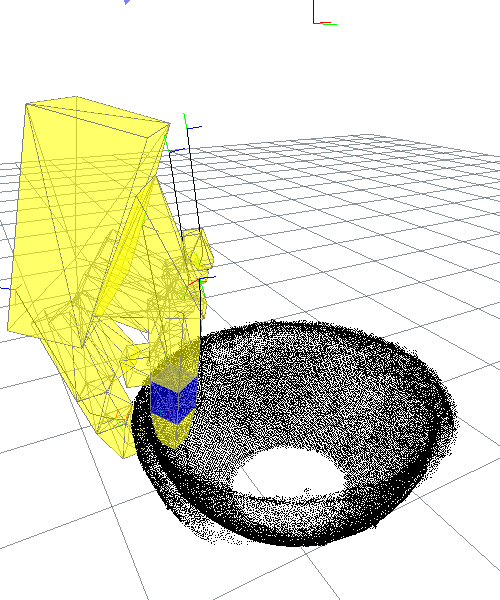
\includegraphics[height=3.5cm]{boris-v7/bowllarge/pinchsupp/link3}
%        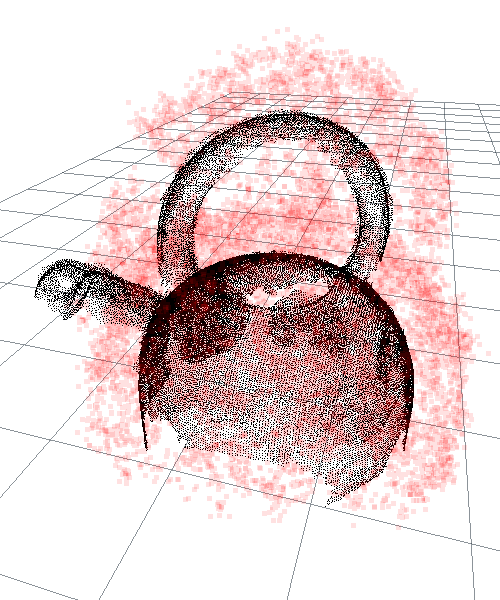
\includegraphics[height=3.5cm]{boris-v7/kettle/pinchsupp/link3-query}
%        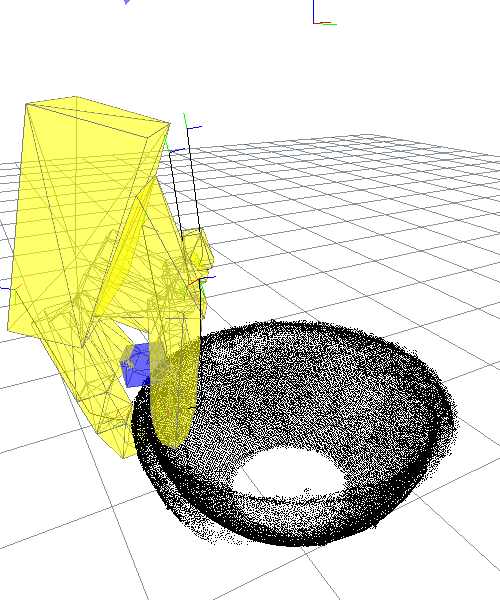
\includegraphics[height=3.5cm]{boris-v7/bowllarge/pinchsupp/link11}
%        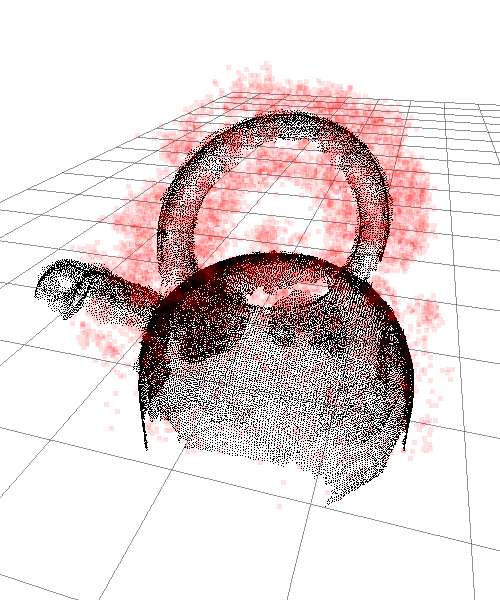
\includegraphics[height=3.5cm]{boris-v7/kettle/pinchsupp/link11-query}
%    }
%    \caption[Query density]{Visualisation of two query densities (panels 2 and 4 from the left) for two contact models (panels 1 and 3) of a pinch with support grasp. The links to which the contact models are associated are in blue. A query density is a distribution over poses of the corresponding link (red cloud) for a new ``query'' kettle.}
%    \label{fig:grasping.querydensity}
%\end{figure}

% experimental work
In experiments with Boris, the training set consisted of five different grasps, and the test set of forty-five previously unseen objects. The success rate of the first choice grasp is 77.7\% using a single view of the test object, and increases to 84.4\% if seven views are taken instead.
%Some example test grasps are given in Figure~\ref{fig:testing}.
%
%% this is Fig.9 of the paper: we could avoid it here
%\begin{figure}[p]
%    \newcommand{\testingw}{0.16\linewidth}
%    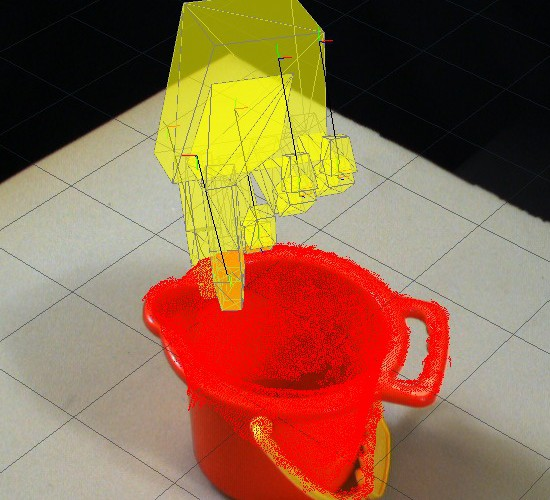
\includegraphics[width=\testingw]{boris-v7-crop/bucket/_cropped_screen000027} 
%    \includegraphics[width=\testingw]{boris-v7-crop/bucket/{_cropped_data-3201.851-externPointGrey.3}.jpg} 
%    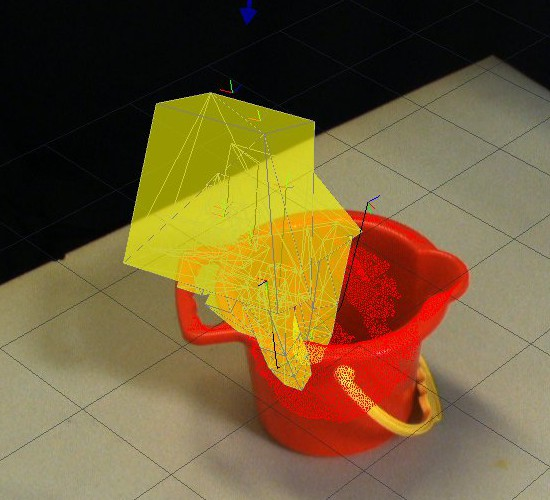
\includegraphics[width=\testingw]{boris-v1-crop/bucket/_cropped_ri} 
%    \includegraphics[width=\testingw]{boris-v1-crop/bucket/{_cropped_datav1-1930.496-externpointgrey3}.jpg} 
%    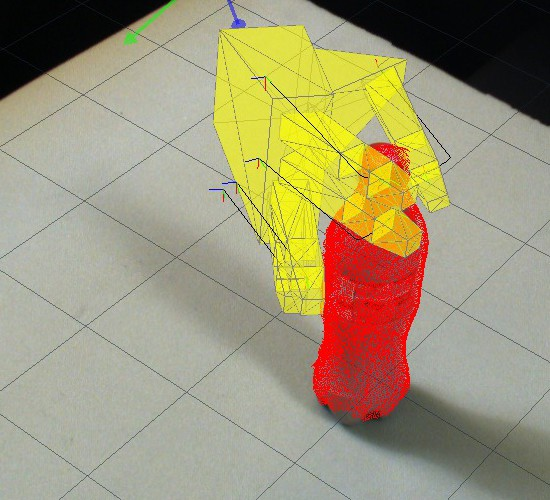
\includegraphics[width=\testingw]{boris-v7-crop/coke/_cropped_screen000051} 
%    \includegraphics[width=\testingw]{boris-v7-crop/coke/{_cropped_data-5546.733-externPointGrey.3}.jpg} 
%    \\
%    \includegraphics[width=\testingw]{boris-v1-crop/coke/_cropped_ri} 
%    \includegraphics[width=\testingw]{boris-v1-crop/coke/{_cropped_datav1-2959.660-externpointgrey3}.jpg} 
%    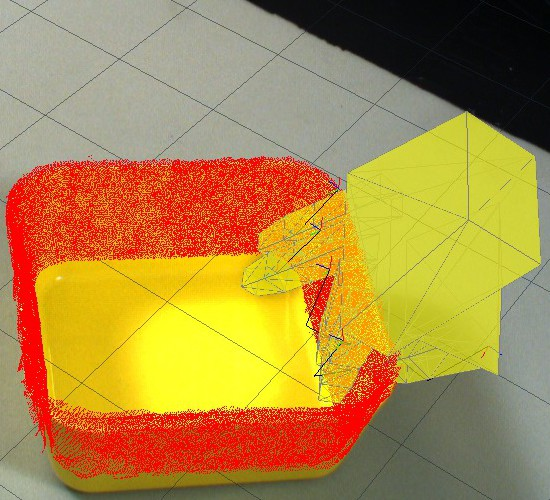
\includegraphics[width=\testingw]{boris-v7-crop/container1/_cropped_screen000016} 
%    \includegraphics[width=\testingw]{boris-v7-crop/container1/{_cropped_data-1839.940-externPointGrey.3}.jpg} 
%    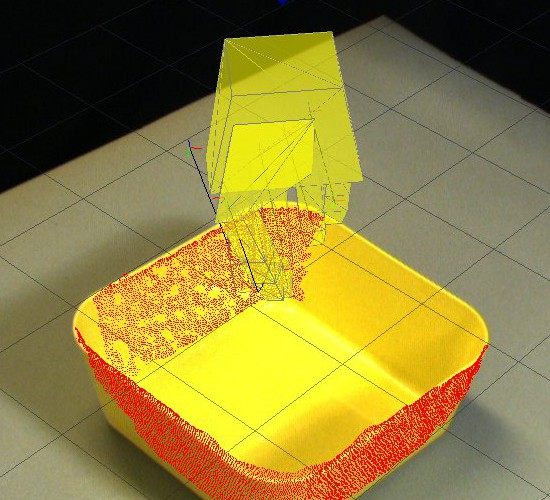
\includegraphics[width=\testingw]{boris-v1-crop/container1/_cropped_ri} 
%    \includegraphics[width=\testingw]{boris-v1-crop/container1/{_cropped_datav1-4038.264-externpointgrey3}.jpg} 
%    \\
%    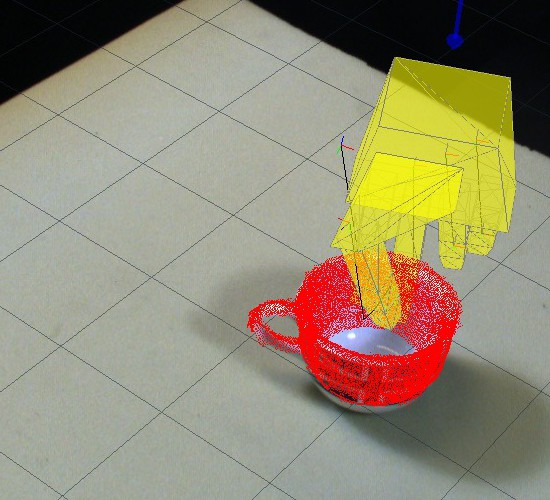
\includegraphics[width=\testingw]{boris-v7-crop/cup2/_cropped_screen000013} 
%    \includegraphics[width=\testingw]{boris-v7-crop/cup2/{_cropped_data-438.213-externPointGrey.3}.jpg} 
%    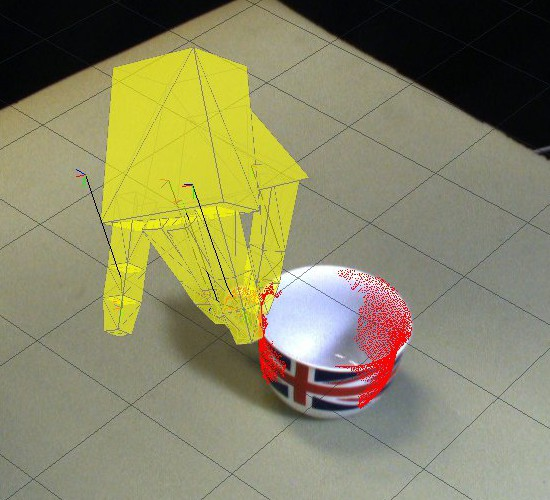
\includegraphics[width=\testingw]{boris-v1-crop/cup2/_cropped_ri} 
%    \includegraphics[width=\testingw]{boris-v1-crop/cup2/{_cropped_datav1-5208.103-externpointgrey3}.jpg} 
%    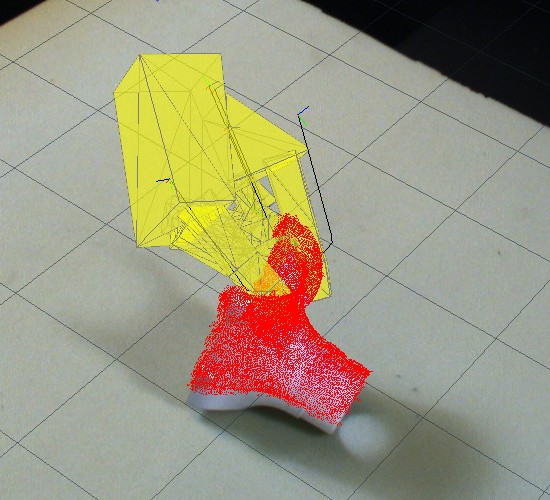
\includegraphics[width=\testingw]{boris-v7-crop/guttering/_cropped_screen000014} 
%    \includegraphics[width=\testingw]{boris-v7-crop/guttering/{_cropped_data2-148.522-externPointGrey.3}.jpg} 
%    \\
%    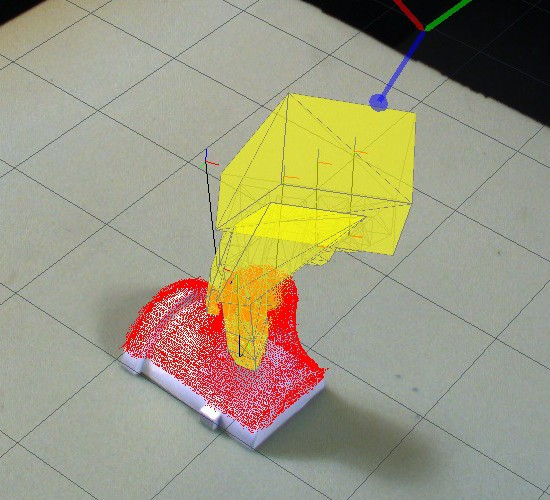
\includegraphics[width=\testingw]{boris-v7-crop/guttering/_cropped_screen000004}
%    \includegraphics[width=\testingw]{boris-v7-crop/guttering/{_cropped_data-585.300-externPointGrey.3}.jpg}
%    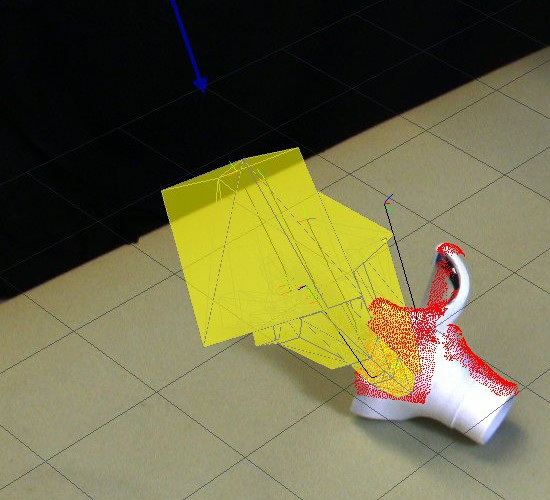
\includegraphics[width=\testingw]{boris-v1-crop/guttering/_cropped_side-gri} 
%    \includegraphics[width=\testingw]{boris-v1-crop/guttering/{_cropped_datav12-5768.286-externpointgrey3}.jpg} 
%    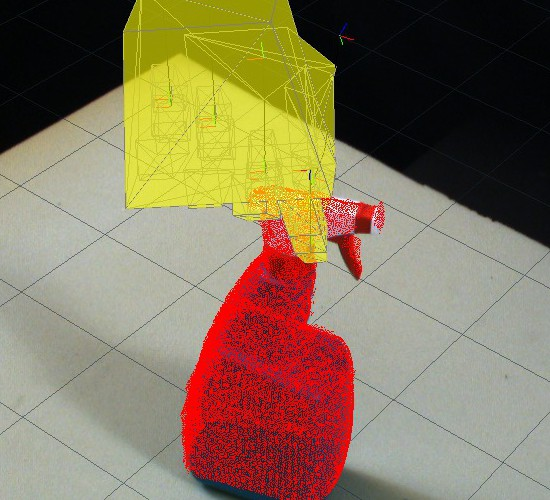
\includegraphics[width=\testingw]{boris-v7-crop/mrmuscle/_cropped_screen000007} 
%    \includegraphics[width=\testingw]{boris-v7-crop/mrmuscle/{_cropped_data-353.435-externPointGrey.3}.jpg} 
%    \\
%    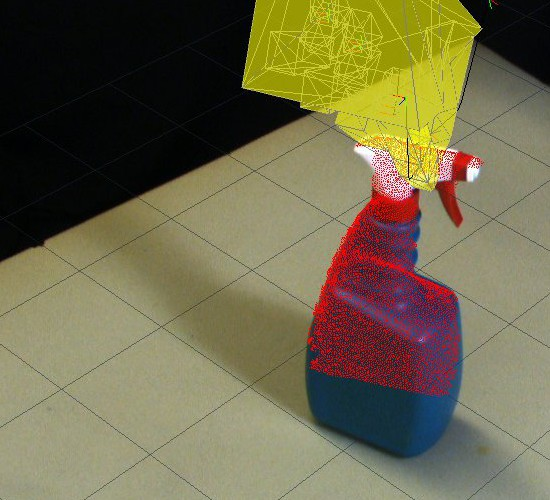
\includegraphics[width=\testingw]{boris-v1-crop/mrmuscle/_cropped_ri} 
%    \includegraphics[width=\testingw]{boris-v1-crop/mrmuscle/{_cropped_datav1-4510.631-externpointgrey3}.jpg} 
%    %\\
%    %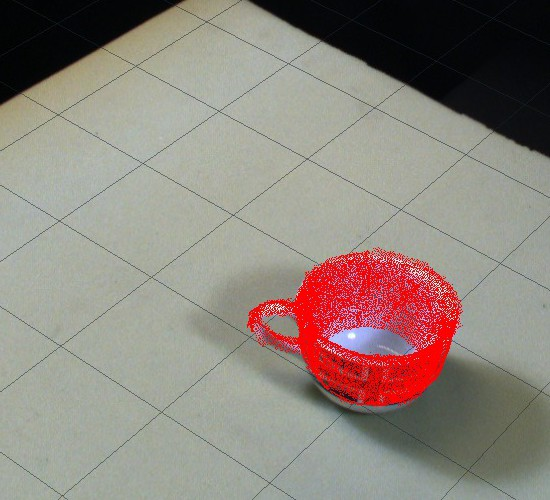
\includegraphics[width=\testingw]{boris-v7-crop/mug1/_cropped_screen000010}
%    %\includegraphics[width=\testingw]{boris-v7-crop/mug1/{_cropped_data2-1739.597-externPointGrey.3}.jpg}
%    %\includegraphics[width=\testingw]{boris-v1-crop/mug1/_cropped_ri}
%    %\includegraphics[width=\testingw]{boris-v1-crop/mug1/{_cropped_datav1-101.071-externpointgrey3}.jpg}
%    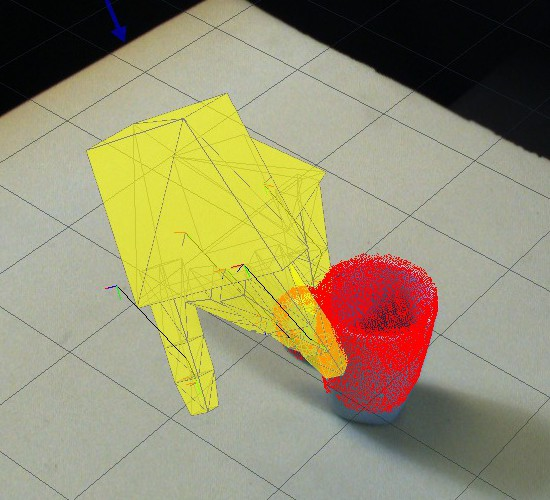
\includegraphics[width=\testingw]{boris-v7-crop/mug4/_cropped_screen000003} 
%    \includegraphics[width=\testingw]{boris-v7-crop/mug4/{_cropped_data-154.877-externPointGrey.3}.jpg} 
%    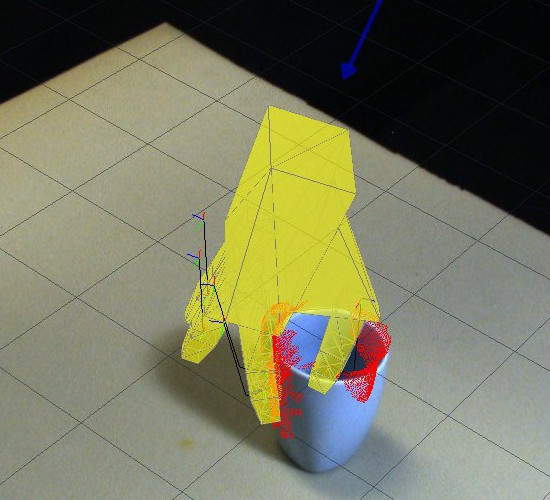
\includegraphics[width=\testingw]{boris-v1-crop/mug4/_cropped_ri} 
%    \includegraphics[width=\testingw]{boris-v1-crop/mug4/{_cropped_datav1-1758.848-externpointgrey3}.jpg} 
%    \\
%    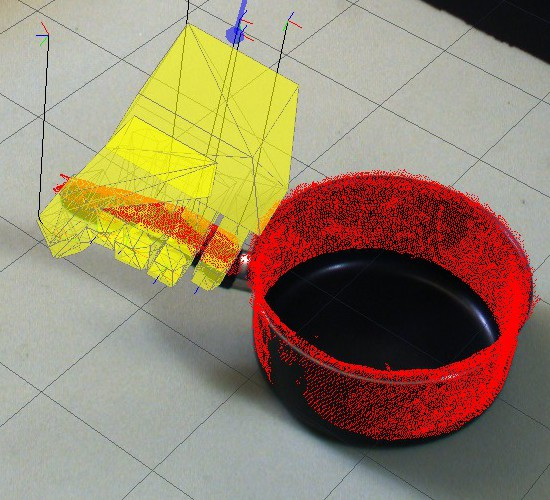
\includegraphics[width=\testingw]{boris-v7-crop/saucepanlarge/_cropped_screen000065}  
%    \includegraphics[width=\testingw]{boris-v7-crop/saucepanlarge/{_cropped_data-3841.539-externPointGrey.3}.jpg}  
%    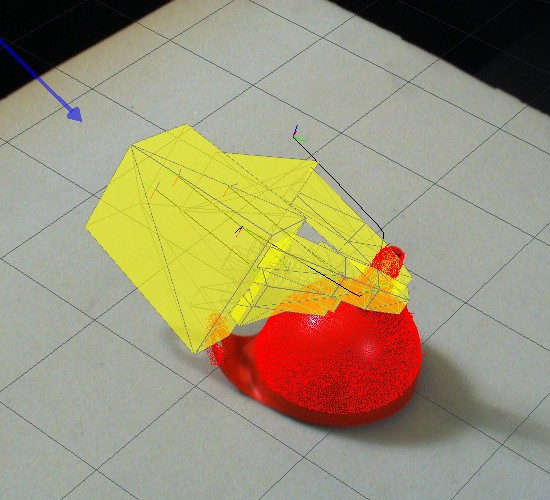
\includegraphics[width=\testingw]{boris-v7-crop/funnellarge/_cropped_screen000038} 
%    \includegraphics[width=\testingw]{boris-v7-crop/funnellarge/{_cropped_data-1856.011-externPointGrey.3}.jpg} 
%    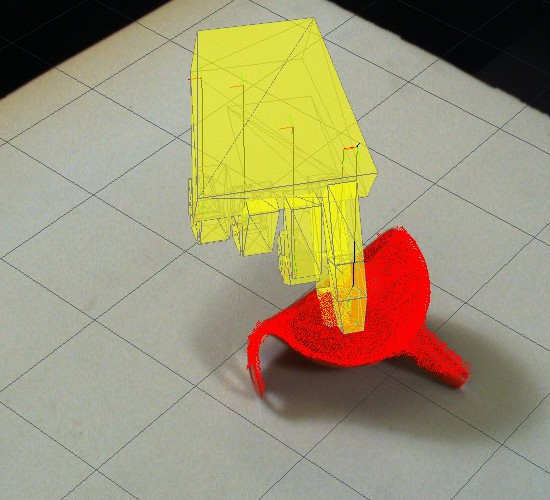
\includegraphics[width=\testingw]{boris-v7-crop/funnellarge/_cropped_screen000054} 
%    \includegraphics[width=\testingw]{boris-v7-crop/funnellarge/{_cropped_data2-3498.448-externPointGrey.3}.jpg} 
%    \\
%    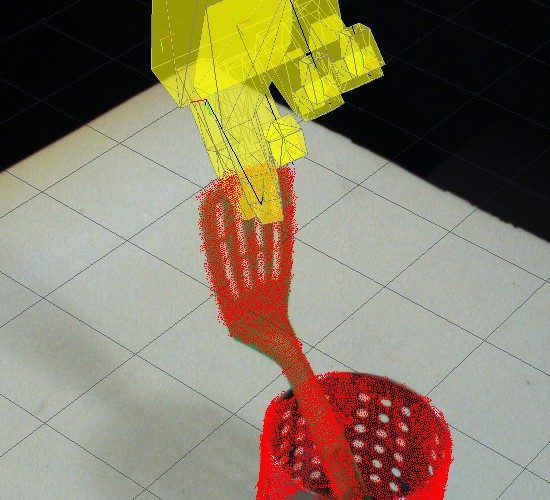
\includegraphics[width=\testingw]{boris-v7-crop/spatula/_cropped_screen000071} 
%    \includegraphics[width=\testingw]{boris-v7-crop/spatula/{_cropped_data3-4065.617-externPointGrey.3}.jpg} 
%    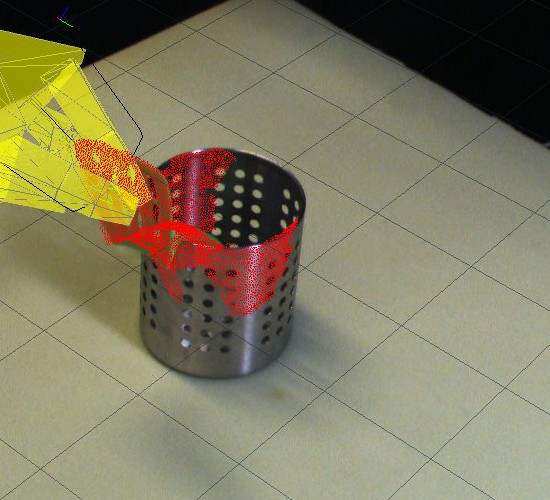
\includegraphics[width=\testingw]{boris-v1-crop/spatula/_cropped_ri} 
%    \includegraphics[width=\testingw]{boris-v1-crop/spatula/{_cropped_datav1-444.576-externpointgrey3}.jpg} 
%    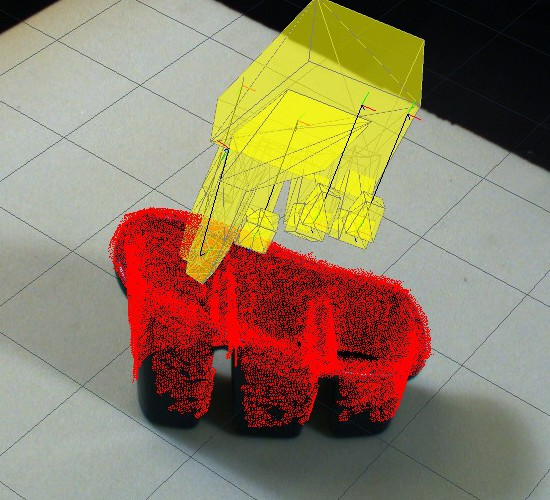
\includegraphics[width=\testingw]{boris-v7-crop/stand1/_cropped_screen000075}  
%    \includegraphics[width=\testingw]{boris-v7-crop/stand1/{_cropped_data-4588.209-externPointGrey.3}.jpg}  
%    \\
%    \includegraphics[width=\testingw]{boris-v1-crop/stand1/_cropped_ri}   
%    \includegraphics[width=\testingw]{boris-v1-crop/stand1/{_cropped_datav1-791.865-externpointgrey3}.jpg}   
%    %\includegraphics[width=\testingw]{boris-v7-crop/tongs/_cropped_screen000054}
%    %\includegraphics[width=\testingw]{boris-v7-crop/tongs/{_cropped_data3-2655.581-externPointGrey.3}.jpg}
%    %\includegraphics[width=\testingw]{boris-v1-crop/tongs/_cropped_ri}
%    %\includegraphics[width=\testingw]{boris-v1-crop/tongs/{_cropped_datav1-874.232-externpointgrey3}.jpg}
%    %\\
%    \includegraphics[width=\testingw]{boris-v7-crop/wineglass/_cropped_screen000042}  
%    \includegraphics[width=\testingw]{boris-v7-crop/wineglass/{_cropped_data-2118.818-externPointGrey.3}.jpg}  
%    \includegraphics[width=\testingw]{boris-v1-crop/wineglass/_cropped_ri}  
%    \includegraphics[width=\testingw]{boris-v1-crop/wineglass/{_cropped_datav1-2051.782-externpointgrey3}.jpg}  
%    \caption{The test objects with a visualisation of some of the successful grasps. Each grasp is shown by a pair of images, with the visualisation of the planned grasp and the obtained point cloud on the left, and the actual grasp execution on the right. Those from the 7 view and 1 view conditions can easily be distinguished by the proportion of the object covered by the recovered point cloud.}
%    \label{fig:testing}
%\end{figure}

More details on the highlighted method and the experimental results can be found in Sec.~\ref{ann:novelObjects}. % available at this~\href{./attachedPapers/GraspingNovelObjects.pdf}{link}. 


%%%%%%%%%%%%%%%%%%%%%%%%%%%%%%%%%%%%%%%%%%%%%%%%%%%%%%%%%%%%%%%%%%%%%%%%%%%%%%

% To be prepared by: UoB (Claudio and Jeremy))
% Grasping under Uncertainty
%%% Grasping under Uncertainty

\subsubsection{Grasping under Uncertainty}
\label{sec:GraspingUncertainty}

 This work extends that of \cite{bib:platt_csail_2011}, which offers a way to avoid the complexity of planning in a high dimensional belief space. It does this in two ways, i) by approximating the informational value of actions from a low-dimensional subspace of the belief state; and ii) by embedding that informational value into the physical space. Whereas Platt employed a 2DoF arm with a laser sensor, our extension allows reasoning about a 21 DoF arm-hand system with tactile observations. 

In our previous work~\cite{bib:zito_workshop_iros2012,bib:zito_iros_2013} we proposed a information gain re-planning strategy to improve the reliability of grasping under uncertainty. We achieved this by using a hierarchical sample-based path planner, here a Probabilistic Roadmap (PRM) planner, which explicitly encodes expected information gain (using a low-dimensional approximation of the belief state) along each of its trajectory segments. This extended the work in~\cite{bib:platt_csail_2011}. A particular contribution of our approach is refining the belief state for the object pose using an observation model for tactile sensing by a multi-finger hand that can palpate the object to be grasped. 

We have extended our previous work in four ways. First we now employ as the target grasp, one of the grasp candidates from the work on grasping of novel objects described elsewhere in this deliverable. Second we now enable re-planning from the configuration of the robot at the point where an unexpected contact occurs. This is instead of moving the hand away from the contact to a safe configuration. Third, we now plan dexterous grasping trajectories for non-convex object shapes by implementing an efficient collision detection method which reasons directly with sensed point clouds rather than derived representations of object shape such as mesh representations. Fourth, we now use an active compliant controller to ensure that continued contact(s) between the hand and the object minimise the risk of perturbing the system.

The updated method has been tested in simulation. Pose uncertainty is now caused by errors in matching a partial point cloud from one or two viewpoints to a previously sensed cloud from seven views. In each trial the simulated robot attempts to grasp the presented object using three different strategies. The first strategy represents a ``naive'' approach in which the robot tries to grasp the object in its estimated pose with a single attempt. The second strategy allows the robot to recover from unexpected contacts if the estimated pose is not correct, and a new grasp attempt is planned and executed until a termination condition is met. The third strategy is teh information gain strategy mentioned above. This works with a cost function that allows deviations from the shortest physical path in order to make tactile contacts that will reduce object pose uncertainty. Essentially this can be seen as warping the physical space using information gain to create a non-Euclidean distance metric
 for motion planning. The goal of the trials is to show that the information gain planner is superior, having a higher success rate, and requiring fewer re-planning iterations than the other methods before a grasp is achieved.


%%%%%%%%%%%%%%%%%%%%%%%%%%%%%%%%%%%%%%%%%%%%%%%%%%%%%%%%%%%%%%%%%%%%%%%%%%%%%%

% To be prepared by: Marco Gabiccini
% Sample-Based Motion Planning for Soft Robot Manipulators
% Under Task Constraints
%%% Sample-Based Motion Planning for Soft Robot Manipulators 
%%% Under Task Constraints

\subsubsection{Sample-Based Motion Planning for Soft Robot Manipulators
Under Task Constraints} 
\label{sec:SampleBasedMotionPlanningSoftRobots}

In this section we present a new sample-based approach to motion planning for soft robot manipulators which considers also task constraints.

As our final goal is to use a bimanual system to grasp and position objects, motion planning cannot neglect the constraints arising from closing the kinematic loop between the two arms, the two hands, and the object being grasped. Moreover, while using compliant manipulators gives new and unforeseen opportunity, it also poses new challenges even on the motion planning side.

Normally, random sampling-based methods for motion planning have the advantage to efficiently sample the robot configuration space (for which we have an explicit parameterization) and may iteratively improve the connection between an initial and a desired final robot configurations.
This advantage deteriorates when we consider constrained motion planning because the lack of an explicit parameterization of the non linear submanifold of the configuration space which satisfies the constraints makes it difficult to find samples which are valid nodes of the plan to be found.
Explicitly, the fraction of the free-from-obstacle configuration space $ \mathcal{M}_{\text{free}} \in \mathbb{R}^{d} $ which strictly satisfies a constraint of the type $ C(q) = 0 $, is a zero-measure submanifold $ \mathcal{M}_{v} $ for which the practical probability of sampling a point $ q \in \mathcal{M}_{v} $ is zero.
Most of the proposed planning methods use projections to generate valid configurations of the system, slowing down the planning process.

Specializing the algorithm for compliant systems, we can avoid this increase in computational burden relaxing the constraint to be of the type $ C(q) \leq \varepsilon $: in the case in which the tight constraint is violated, a force proportional to the violation arises between two parts in contact, but still the configuration is feasible (although undesired forces on the grasped object could be generated).
In this way, we can sample a boundary layer $ \mathcal{M}_{r} := \{q \in \mathcal{M}_{\text{free}},\,C(q)\leq \varepsilon \} $ which has the same dimensionality as the whole configuration space, and volume decreasing with $ \varepsilon $.
We can then use a biased random sampling technique like the one in \cite{bialkowsky2013free}, which allows us to obtain a sample distribution which tends to be uniform in $ \mathcal{M}_{r} $.

Once the planning problem is solved, the main challenge arises from the fact that the relaxed constraint has now to be enforced during execution in order to avoid undesired forces acting on the object.
This has to be ensured via a real-time controller, which can be synthesised exploiting the geometric formulation introduced in \cite{prattichizzo1997consistent,prattichizzo1998dynamic} where an algorithm to make the position and force control of certain systems non-interacting has been devised, allowing for regulating internal object forces to an appropriate level without jeopardising the planned motion.

More details on this new approach and on the currently achieved results can be found in the attached paper~\cite{bonilla2015samplebased} available at this~\href{./attachedPapers/SampleBasedMotionPlanningSoftRobots.pdf}{link}. 

%%%%%%%%%%%%%%%%%%%%%%%%%%%%%%%%%%%%%%%%%%%%%%%%%%%%%%%%%%%%%%%%%%%%%%%%%%%%%%

% To be prepared by: Marco Gabiccini
% Integrated Constrained Motion Planning and Control for
% Compliant Robots
%%%% Integrated Constrained Motion Planning and Control for
%%% Compliant Robots

\subsubsection{Integrated Constrained Motion Planning and Control for
Compliant Robots}
\label{sec:ConstrainedMotionPlanningAndControl} 

%%%%%%%%%%%%%%%%%%%%%%%%%%%%%%%%%%%%%%%%%%%%%%%%%%%%%%%%%%%%%%%%%%%%%%%%%%%%%%

% To be prepared by: Hamal Marino
% High-Level Planning for Dual Arm Goal-Oriented Tasks
%%% High-Level Planning for Dual Arm Goal-Oriented Tasks

\subsubsection{On the Problem of Moving Objects with Autonomous Robots: a Unifying High-Level Planning Approach}
\label{sec:HighLevelPlanning}

In order to successfully complete Task~5.3, which requires the object to be passed between the hands of the robot, we describe in this section our approach to solve high-level planning for this matter.

Our idea considers the possibility of having the object in a known position, which can be recognized using vision, and a higher-level agent (such as a user) decides a target configuration the object has to reach.

From this information, a semantic graph is constructed which has as nodes a grasp id and a workspace id, and as arcs all possible known transitions between nodes.

Once a minimum cost path has been found, it is translated back into Cartesian information for collision-free motion planning, grasp commands, and all low-level requirements to execute the plan successfully.

While there are many previous works on combining high-level semantic reasoning and low-level cartesian path planning (see e.g. \cite{karlsson2012combining, leidner2012things, leidner2013hybrid}) which mostly take advantage of object-specific reasoning introduced in \cite{levison1996connecting}, our main contribution is to include the possibility of passing an object between two end-effectors.

Specifically, considering end-effectors with different properties, the table (and possibly other non-movable surfaces) has its own set of grasps for an object, and is treated exactly like a hand when generating arcs in the graph, apart from the fact that it cannot be moved and, thus, there will be no arc connecting the same ``table grasp'' in adjacent workspaces (while there could be one if the grasp is performed via a hand of the robot).

Thus, considering that previous approaches mostly rely on a table in order to move an object from one arm workspace to another, we can simply classify the \emph{primitives} which allow a transition from a grasp/workspace pair into another in three categories:
\begin{enumerate}
	\item \emph{pick} with an end-effector from a fixed surface
	\item \emph{move} the end-effector
	\item \emph{place} with an end-effector onto a fixed surface
\end{enumerate}

Our approach uses instead a more general action of ``grasp transfer'', which can be specialized in:
\begin{enumerate}
	\item moving actions of an end-effector among its reachable workspaces
	\item pick and place actions if one end-effector involved is non-movable (such as a table)
	\item a grasp-ungrasp sequence if both end-effectors involved are movable
\end{enumerate}
This list is still under development, and we will try to generalize it even more in the future with other, more interesting \emph{primitives} which could possibly exploit dynamics, friction, gravity, and so on.

A more detailed view on this method and on the achieved results can be seen in Sec.~\ref{ann:highLevelPlanning}. % available at this~\href{./attachedPapers/HighLevelPlanningBimanualObjectPassing.pdf}{link}.


%%%%%%%%%%%%%%%%%%%%%%%%%%%%%%%%%%%%%%%%%%%%%%%%%%%%%%%%%%%%%%%%%%%%%%%%%%%%%%

% To be prepared by: Marco Gabiccini
% Computational Framework for Environment-Aware Robotic Manipulation
% Planning
%%% A Computational Framework for Environment-Aware Robotic Manipulation 
%%% Planning

\subsubsection{A Computational Framework for Environment-Aware Robotic Manipulation Planning}

Moving beyond with respect to what we committed to investigate in Tasks 4.2 and 4.3, we introduce, in this section, a computational framework for direct trajectory optimization of general manipulation systems without \textsl{a-priori} specified contact sequences, possibly exploiting \emph{environmental constraints} as a tool to accomplish a task.
 
 Originally, we planned to approach the problem of robust grasping by dividing it into three main stages: (i) move from hand pre-shape to first object contact (Task 4.1), (ii) perform an incipient grasp and assess the first-order properties of the surface of the object, possibly changing candidate contact locations so that the quality of the incipient grasp is maximized (Task 4.2), and (iii) perform the actual grasp acquisition by optimizing the distribution of the applied contact forces (Task 4.3).
 
 In this section, we report on our efforts to devise a framework to be employed not only for grasp planning, but also for manipulation planning, that should be able to merge all three previous phases in a systematic and coherent way. The user should be focused on providing high-level objectives, e.g. ``move object A from pose 1 to pose 2 in a given amount of time'', and the framework should be able to provide a manipulation plan that should take care of all the rest, e.g. should specify low-level actions and their correct sequence for the manipulation system at hand (single-arm configuration, dual-arm configuration),  defining the whole contact sequence (where and when to make and to break contacts), should provide trajectories consistent with the dynamics of the manipulation system, unilateral contact and friction constraints and actuation limits. Then, if the task may be more efficiently, and/or more robustly, performed with the aid of constraints provided by the environment, the proposed approach should devise manipulation strategies that cleverly and opportunistically exploit environmental constraints.
 
 To this sake, two approaches are presented to model the dynamics of systems with intermittent contacts: the first one, in which continuous contact reaction forces are generated  by nonlinear virtual springs, is convenient to tackle scenarios where we try to avoid \emph{sliding} contacts; the second one, which is based on a velocity-based time stepping scheme, is suitable in scenarios where \emph{sliding} interaction primitives may lead to convenient interactions among the hand, the manipulandum and the environment.

In both cases, beside system's state and applied torques, object and environment contact forces are included among the free optimization variables, and they are rendered consistent via suitably devised sets of \emph{complementarity} conditions. To maximize computational efficiency, sparsity patterns in the linear algebra expressions generated during the solution of the optimization problem are exploited, and Algorithmic Differentiation (also known as Automatic Differentiation) is leveraged to calculate derivatives. 

The approach is evaluated in three simulated planar manipulation tasks: (i) moving a circular object from an initial pose to a final pose in the workspace with two independent fingers, (ii) rotating a capsule-shaped object with an underactuated two-fingered gripper, and (iii) rotating a circular object in hand with three independent fingers. Tasks (i) and (ii) show that our algorithm quickly converges to locally optimal solutions that opportunistically exploit environmental constraints. Task (iii) demonstrates that even dexterous fingertip gaits can be obtained as a special solution in the very same framework.

More details on this new approach and on the achieved results can be found in the attached paper~\cite{Gabiccini:RSS:2015} available at this~\href{./attachedPapers/ComputationalFrameworkEnvAwareRobManipPlanning.pdf}{link}. 

%%%%%%%%%%%%%%%%%%%%%%%%%%%%%%%%%%%%%%%%%%%%%%%%%%%%%%%%%%%%%%%%%%%%%%%%%%%%%%
\newpage

\bibliographystyle{IEEEtran}
\bibliography{../shared_bibliography/abbreviations,./bibliography/DR42}

\newpage

\appendix
\section{Annexes}

\subsection{Article: Grasping with soft hands} \label{ann:softGrasps}
\begin{description}
    \item[Authors] M. Bonilla, E. Farnioli, C. Piazza, M. Catalano, G. Grioli, M. Garabini, M. Gabiccini, A. Bicchi
    \item[Info] In proceedings of IEEE-RAS Int. Conf. on Humanoid Robots (Humanoids), 2014
    \item[Abstract] Despite some prematurely optimistic claims, the ability of robots to grasp general objects in unstructured environments still remains far behind that of humans. This is not solely caused by differences in the mechanics of hands: indeed, we show that human use of a simple robot hand (the Pisa/IIT SoftHand) can afford capabilities that are comparable to natural grasping. It is through the observation of such human-directed robot hand operations that we realized how fundamental in everyday grasping and manipulation is the role of hand compliance, which is used to adapt to the shape of surrounding objects. Objects and environmental constraints are in turn used to functionally shape the hand, going beyond its nominal kinematic limits by exploiting structural softness. In this paper, we set out to study grasp planning for hands that are simple - in the sense of low number of actuated degrees of freedom (one for the Pisa/IIT SoftHand) - but are soft, i.e. continuously deformable in an infinity of possible shapes through interaction with objects. After general considerations on the change of paradigm in grasp planning that this setting brings about with respect to classical rigid multi-dof grasp planning, we present a procedure to extract grasp affordances for the Pisa/IIT SoftHand through physically accurate numerical simulations. The selected grasps are then successfully tested in an experimental scenario.
    \item \textbf{Relation with the deliverable}: Grasping under uncertainty by exploiting the adaptive behavior encoded in the mechanical design.
    \item[Attachment] (following pages until next annex)
\end{description}
\includepdf[pages=-]{./attachedPapers/GraspingWithSoftHands.pdf}

\subsection{Article: Grasp Planning for the Pisa/IIT Softhand via Bounding-Box Object Decomposition} \label{ann:boxedGrasp}
\begin{description}
    \item[Authors] M. Bonilla, D. Resasco, M. Gabiccini, A. Bicchi
    \item[Info] Under review
    \item[Abstract] In this paper we present a method to plan grasps for Soft Hands. Considering that Soft Hands adapt to the shape of the object whatever its geometry is, we first approximate the object with bounding boxes. A set of hand poses are then proposed using geometric information of such bounding boxes. All hand postures are then used in a dynamic simulator of the PISA/IIT Soft Hand to evaluate if a proposed hand posture leads to a successful grasp or not.
    We show through a set of simulations that the probability of success of the proposed hand poses is higher that with the existing methods.
    At the end we show some experimental work using the PISA/IIT Soft Hand.
    \item[Relation with the deliverable] Part-based grasping under uncertainty for soft hands.
    \item[Attachment] (following pages until next annex)
\end{description}
%% TO BE INCLUDED
%\includepdf[pages=-]{./attachedPapers/.pdf}

\subsection{Article: One shot learning and generation of dexterous grasps for novel objects} \label{ann:novelObjects}
\begin{description}
    \item[Authors] M. Kopicki, M. Adjible, R. Stolkin, A. Leonardis, R. Detry, J.L. Wyatt
    \item[Info] Under review
    \item[Abstract] This paper presents a method for one-shot learning of dexterous grasps, and grasp generation for novel objects. A model of each grasp type is learned from a single kinesthetic demonstration, and several types are taught. These models are used to select and generate grasps for unfamiliar objects. Both the learning and generation stages use an incomplete point cloud from a depth camera – no prior model of object shape is used. The learned model is a product of experts, in which experts are of two types. The first is a contact model and is a density over the pose of a single hand link relative to the local object surface. The second is the hand configuration model and is a density over the whole hand configuration. Grasp generation for an unfamiliar object optimises the product of these two model types, generating thousands of grasp candidates in under 30 seconds. The method is robust to incomplete data at both training and testing stages. When several grasp types are considered the method selects the highest likelihood grasp across all the types. In an experiment, the training set consisted  of five different grasps, and the test set of forty-five previously unseen objects. The success rate of the first choice grasp is 84.4\% or 77.7\% if seven views or a single view of the test object are taken, respectively.
    \item[Relation with the deliverable] A new method is proposed for learning grasps and generalize them to novel objects.
    \item[Attachment] (following pages until next annex)
\end{description}
\includepdf[pages=-]{./attachedPapers/GraspingNovelObjects.pdf}

% grasping under uncertainty
% \subsection{Book chapter/Article/Technical Report: \em TITLE grasping under uncertainty} \label{ann:uncertaintyGrasps}
% \begin{description}
%     \item[Authors] \em AUTHORS
%     \item[Info] \em UNDER REVIEW / IN PRESS / ACCEPTED FOR PUBLICATION (PROVIDE WHERE) / PUBLISHED AND AVAILABLE ONLINE (PROVIDE DOI)
%     \item[Abstract] \em ABSTRACT
%     \item \textbf{Relation with the deliverable}: \em SELF EXPLAIN
%     \item[Attachment] (following pages until next annex)
% \end{description}
% to be included
%\includepdf[pages=-]{./attachedPapers/GraspingNovelObjects.pdf}

\subsection{Article: Sample-based motion planning for soft robot manipulators under task constraints} \label{ann:softPlanning}
\begin{description}
    \item[Authors] M. Bonilla, E. Farnioli, L. Pallottino, A. Bicchi
    \item[Info] Accepted for publication at the 2015 IEEE Int. Conf. on Robotics and Automation
    \item[Abstract] Random sampling-based methods for motion planning of constrained robot manipulators has been widely studied in recent years. The main problem to deal with is the lack of an explicit parametrization of the non linear submanifold in the Configuration Space (CS), due to the constraints imposed by the system. Most of the proposed planning methods use projections to generate valid configurations of the system slowing the planning process. Recently, new robot mechanism includes compliance either in the structure or in the controllers. In this kind of robot most of the times the planned trajectories are not executed exactly by the robots due to uncertainties in the environment. Indeed, controller references are generated such that the constraint is violated to indirectly generate forces during interactions. In this paper we take advantage of the compliance of the system to relax the geometric constraint imposed by the task, mainly to avoid projections. The relaxed constraint is then used in a state-of-the-art sub-optimal random sampling based technique to generate any-time paths for constrained robot manipulators. As a consequence of relaxation, contact forces acting on the constraint change from configuration to configuration during the planned path. Those forces can be regulated using a proper controller that takes advantage of the geometric decoupling of the subspaces describing constrained
    rigid-body motions of the mechanism and the controllable forces.
    \item[Relation with the deliverable] planning dual arm manipulation for soft robots.
    \item[Attachment] (following pages until next annex)
\end{description}
\includepdf[pages=-]{./attachedPapers/SampleBasedMotionPlanningSoftRobots.pdf}

% \subsection{Article: Integrated Constrained Motion Planning and Control for Compliant Robots} \label{ann:controlledSoftPlanning}
% \begin{description}
%     \item[Authors]
%     \item[Info] Submitted to the 2015 IEEE/RSJ Int. Conf. on Intelligent Robots and Systems
%     \item[Abstract]
%     \item[Relation with the deliverable]
%     \item[Attachment] (following pages until next annex)
% \end{description}
%\includepdf[pages=-]{./attachedPapers/.pdf}

\subsection{Article: High-Level Planning for Dual Arm Goal-Oriented Tasks} \label{ann:dualArmPlanning}
\begin{description}
    \item[Authors] H. Marino, M. Ferrati, A. Settimi, C. Rosales, M. Gabiccini
    \item[Info] under review
    %Submitted to the 2015 IEEE/RSJ Int. Conf. on Intelligent Robots and Systems
    \item[Abstract] 
    In this paper we design a simple methodology for high-level planning, corroborated by low-level planning and simulated execution, of a task to be solved given a set of ``interaction primitives''. We exemplify this with the simple task of moving an object from a given initial to a desired final configuration, possibly, and opportunistically, by exploiting the interaction between the object and the tabletop; here the interaction primitives are the different ways in which the object can be grasped and moved around, possibly different for each end-effector, and the planning step is carried out considering the table itself as an end-effector (with a ``non-movable'' attribute) with its own set of primitives.
    
In this way, we can avoid an excessive increase in computational burden for the planning step, considering that each object has a pre-defined set of primitives for different end-effectors, and that transitions between states can only happen in a pre-defined manner. Such a database can be generated via experiments, simulations, or direct exploration of the environment when new objects are encountered.
    \item[Relation with the deliverable] passing objects from one hand to another (Task 5.3)
    \item[Attachment] (following pages until next annex)
\end{description}
%\includepdf[pages=-]{./attachedPapers/.pdf}

\subsection{Article: A computational framework for environment-aware robotic manipulation planning} \label{ann:env-awareManipulation}
\begin{description}
    \item[Authors] M. Gabiccini, A. Artoni, G. Pannocchia, J.~Gillis
    \item[Info] Under review
    \item[Abstract] In this paper, we present a computational framework for direct trajectory optimization of general manipulation systems with unspecified contact sequences, exploiting \emph{environmental constraints} as a key tool to accomplish a task.
    Two approaches are presented to describe the dynamics of systems with contacts, which are based on a penalty formulation and on a velocity-based time-stepping scheme, respectively. In  both cases, object and environment contact forces are included among the free optimization variables, and they are rendered consistent via suitably devised sets of complementarity conditions.
    To maximize computational efficiency, we exploit sparsity patterns in the linear algebra expressions generated during the solution of the optimization problem and leverage Algorithmic Differentiation to calculate derivatives. % quickly and accurately.
    The benefits of the proposed methods are evaluated in three simulated planar manipulation tasks, where essential interactions with environmental constraints are automatically synthesized and opportunistically exploited.
    \item[Relation with the deliverable] grasp and manipulation planning for systems with a-priori unspecified contact sequences.
    \item[Attachment] (following pages until next annex)
\end{description}
\includepdf[pages=-]{./attachedPapers/ComputationalFrameworkEnvAwareRobManipPlanning.pdf}
\includepdf[pages=-]{./attachedPapers/appendix_of_ComputationalFrameworkEnvAwareRobManipPlanning.pdf}

\end{document}
